\section{Component Selection}

\subsection{Analog Controllers \& Components}

We are utilizing a single analog controller in the project for a highly flexible, efficient and feature-packed converter. The main controller selected for these operations is UCC28740 Constant-Voltage Constant-Current Flyback Controller
Using Optocoupled Feedback by Texas Instruments. It will be powered by an auxiliary winding wound to the transformer. It is designated to be always used in DCM operation. It can take feedback from both primary and secondary sides and can keep output voltage constant and performs well in load and line regulation aspects. It has an embedded MOSFET driver to save space lower the component count. Furthermore, its internal algorithm also provides soft-switching to lower the initial stresses on the components.

This controller IC is directly designed by Texas Instruments to control the isolated Flyback Converters. It provides Constant-Voltage (CV) using an optical coupler to improve transient response to large load steps. It also accomplishes Constant-Current (CC) regulation through Primary-Side-Regulation (PSR) techniques. It processes the information taken from opto-coupled feedback and the auxiliary flyback winding, and uses this processed information to achieve precise high-performance control of the output voltage and current of the converter. The control algorithms used in this IC helps it to achieve high efficiency levels. The DCM operation with the valley switching technique reduces the switching losses, and hence increases the overall efficiency.

The selected controller has a maximum switching frequency of 100 kHz, and always maintains the control of the peak primary current in the transformer. Furthermore, the embedded protection features help to keep the primary and secondary component stresses of the converter in check.

A reference design schematic for the selected controller IC UCC28740 is shown in Figure \ref{fig:analog_cont}, below.

\begin{figure}[H]
\centering
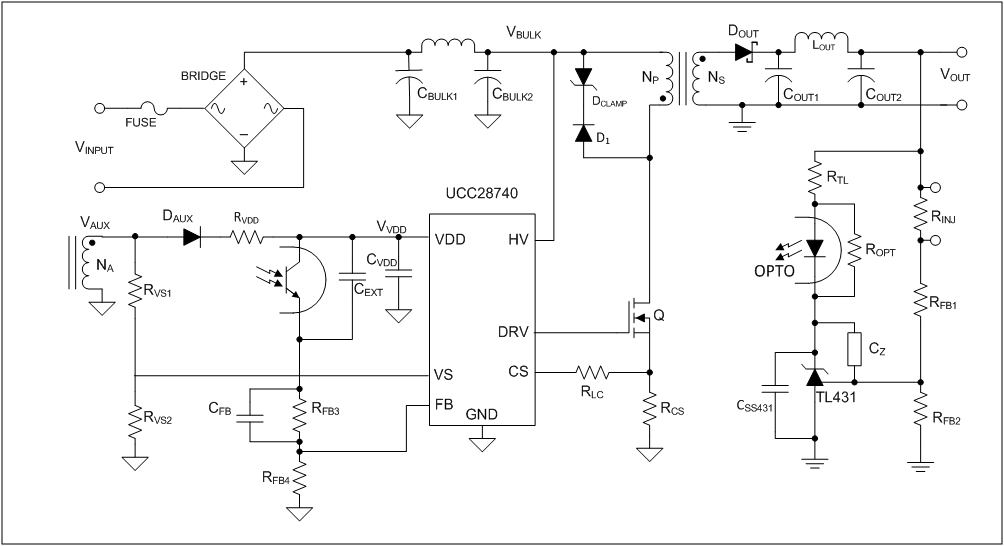
\includegraphics [width=0.8\textwidth]{figures/Analog_Controller.png}
\caption{Flyback Controller Reference Design with UCC28740}
\label{fig:analog_cont}
\end{figure}

\subsection{MOSFET Selection}
For the MOSFET selection, we need to consider the maximum voltage and current stresses over the MOSFET.

The maximum voltage stress over the MOSFET is obtained analytically by the following relation.

$$ V_{sw,peak} = V_{in,max} + \frac{N_P}{N_S}V_{out} $$

where $ V_{in,max} = 48\;V $, $ V_{out} = 15\;V $ and $ \frac{N_P}{N_S} = 1.9 $.

Then, the peak voltage over the MOSFET is computed analytically as follows:

$$ V_{sw,peak} = 48 + 1.9*15 = 76.5\;V $$

This value is in parallel with the peak voltage value obtained from the simulations of the ideal Flyback Converter circuit in Simulink.

The maximum current stress over the MOSFET is obtained analytically by the following relation.

$$ I_{sw,peak} = \frac{1}{(1-D)}\frac{N_S}{N_P}I_o + \frac{N_P}{N_S}\frac{(1-D)T_s}{2L_m}V_o $$

where $ I_o = \frac{P_o}{V_o} = \frac{60}{15} = 4\;A $

Then, the peak MOSFET current is found as follows:

$$ I_{sw,peak} = \frac{1}{(1-0.26)}*\frac{1}{1.9}*4 + 1.9*\frac{(1-0.26)*(1/45000)}{2*28.67*10^{-6}}*15 = 11\;A$$

One thing to notice here is that this peak current is computed assuming CCM operation. However, in our design, the converter mostly operates in DCM as seen from the voltage and current figures presented in the Simulation Results part. Therefore, for the MOSFET peak current value, we need to rely on the simulation results.

However, due to the leakage inductance of the designed transformer, the voltage and current stress over the MOSFET increases. The leakage inductance of the primary winding of the transformer causes voltage spikes over the MOSFET due to the instant changes in inductor current, $di_L/dt$, which in result causes switch failures. In order to prevent giving undesirable damages to the MOSFET, we designed an RCD snubber to provide a safe discharging path for the transformer primary leakage inductance over itself and RC circuit of the snubber. 

From the simulations of the Flyback Converter circuit in Simulink, the MOSFET peak voltage and current are measured as $ V_{sw,peak} = 300\;V $ $ I_{sw,peak} = 10\;A $

Overall, the peak voltage and current ratings for the MOSFET are found as follows:

$$ V_{sw,peak} = 300\;V $$
$$ I_{sw,peak} = 10\;A $$
$$ I_{sw,mean} = 2.84\;A $$
$$ I_{sw,RMS} = 4.366\;A $$

The selected MOSFET should also be able to handle the switching frequencies as high as 45 kHz. 
Since it is a very commonly used value, choosing a 400V MOSFET is reasonable. STP17NK40ZFP by STMicroelectronics is a good choice since it has current rating of 15A continuous, has a low ON resistance and costs relatively low.

\textbf{Selected Switch: } \href{https://pdf1.alldatasheet.com/datasheet-pdf/view/24337/STMICROELECTRONICS/STP17NK40ZFP.html}{STP17NK40ZFP}

Some important parameters for the selected switch are as follows:

\textbf{Switch Parameters}

\begin{itemize}
    \item $V_{DS} = 400V$
    \item $I_{DS} = 15A\;(@\; T_C = 25\degree C)$
    \item $I_{DS} = 9.4A\;(@\; T_C = 100\degree C)$
    \item $R_{DS_{(on)}} = 0.25\ohm\;(max)$
    \item $V_{GS(th)} = 3.75V\;(typ.)$
    \item Diode Forward Voltage: $V_{SD,forward} = 1.6V$\;(max)
    \item Diode Forward Current: $I_{SD} = 15A$
    \item Price: 3.34\$
\end{itemize}

\subsection{Diode Selection}
Similar to the MOSFET selection, the maximum voltage and current stresses over the diode must be determined for the diode selection.

The maximum reverse voltage across the diode during its off period can be calculated as
\begin{align*}
    V_D=V_{out}+N_{PS}V_{in,max}=-40.26V
\end{align*}

It is observed to be $ V_{diode,peak} = -40.26\;V $ from the simulations.

The maximum forward current through the diode during its on period can be calculated as:
\begin{align*}
    I_{s,peak}=\frac{2P_{out}}{D_{MAG}V_{OUT}}=18.89A
\end{align*} 

It is observed to be $ I_{diode,peak} = I_{s,peak} = 19.89\;A $ from the simulations.

Overall, the peak voltage and current ratings for the diode are found as follows:

$$ V_{diode,peak} = -40.26\;V $$
$$ I_{diode,peak} = 19.89\;A $$
$$ I_{diode,mean} = 4.019\;A $$
$$ I_{diode,RMS} = 7.30\;A $$

Also, it should be noted that the average current of the diode will be equal to the average output current, which is 4A. Therefore, MBR10100G from ON Semiconductor is chosen which is a Fast Recovery Schottky diode with 100V and 10A continuous voltage and current ratings diode, which is quite suitable for the given converter application, and the rated operation of our Flyback Converter circuit.

\textbf{Selected Diode: } \href{https://www.onsemi.com/pub/Collateral/MBR1080-D.PDF}{MBR10100G}

Some important parameters for the selected diode are as follows:

\textbf{Diode Parameters}

\begin{itemize}
    \item Type: Schottky Barrier
    \item $V_{RRM} = 100V$
    \item $I_{F(AV)} = 10A\; (@\; T_C = 133\degree C)$
    \item $I_{FRM} = 20A\; (@\; T_C = 133\degree C)$
    \item $I_{FSM} = 150A$
    \item $I_{RRM} = 0.5A$
    \item $V_F = 0.7V\;(@\;i_F = 10A,\; T_C = 125\degree C)$
    \item $I_R = 6mA$
    \item $T_J = -65\;to\;+175\degree C$
    \item $R_{\theta JC} = 2.0\degree C/W$
    \item $R_{\theta JA} = 60\degree C/W$
    \item $R_{ON} = 0.1\ohm\;(@\;i_F = 4A,\;T_C = 150\degree C)$
    \item Price: 0.85\$
\end{itemize}

\subsection{Output Capacitor Selection}
The average voltage across the output capacitor is equal to the average output voltage.

$$ V_{cap,avg} = V_{out} = 15\; $$

Then, the rated voltage of the selected capacitor must be greater than 15 V.

$$ V_{cap,rated} > 15\;V $$

One another limitation on the capacitor selection is the peak-to-peak output voltage ripple limit of the project. The peak-to-peak output voltage ripple is required to be less than 4\%.

$$ \frac{\Delta V_o }{V_o} = 0.04\;(4\%) $$

Then, the maximum allowable output voltage ripple is found as:

$$ \Delta V_o = 0.04*15\;V = 0.6\;V $$ 

Also, let's calculate the maximum allowable ESR for the required ripple.
\begin{align*}
    ESR_{C_{OUT}}=\frac{0.9V_ripple}{I_{s,max}}=20m\Omega
\end{align*}
The output voltage ripple for the Flyback Converter topology is computed from the following relation.

$$ \frac{\Delta V_o }{V_o} = \frac{DT_s}{RC} = \frac{D}{RCf_s} $$

Then, the minimum required output capacitance value is obtained as follows:

$$ C_{min} = \frac{D}{0.04*R*f_s} $$

where $ R = \frac{V_o^2}{P_o} = \frac{15^2}{60} = \frac{225}{60} = 3.75\;\ohm $

$$ C_{min} = \frac{0.26}{0.04*3.75*45000} = 77.8\;\micro F $$

Also, let's calculate the maximum allowable ESR for the required ripple.

\begin{align*}
    ESR_{C_{OUT}}=\frac{0.9V_ripple}{I_{s,max}}=20m\Omega
\end{align*}

We need to select an output capacitor with a rated voltage above 15 V and capacitance value higher than 77.8 \micro F. In addition, the ESR rating of the selected capacitor should also be as small as
possible in order to minimize the voltage drop in the average output voltage level. It is also required to have a small ESR value capacitor in order to keep the converter efficiency as high as possible by minimizing the losses.

Since it is either hard to find or very costly, using ceramic capacitors is not reasonable. Instead, using electrolytic capacitor is a good idea. However, since ESR generally increases with lower capacitance a good balance needs to be found.

Ceramic capacitors are a good choice since their ESR value are quite small compared to aluminum electrolytic capacitors. But, they have the drawback of generally having much higher prices than the aluminum electrolytic capacitors.This creates the compromise or the trade-off between the two types of capacitors. However, since it is difficult to find a small capacitor with the required capacitance value, which is also able to carry the given output current ripple, we decided to use a small aluminum electrolytic capacitor with small ESR rating. It is easier to find small ESR rated aluminum electrolytic capacitors with small capacitance values, which are also able to carry high ripple current values.

Therefore, we decided to select the EEE1HA211P part numbered aluminum electrolytic capacitor (SMD type) of Panasonic. Its rated voltage and current values meets the specifications of our Flyback Converter circuit.

\textbf{Selected Capacitor: } \href{https://media.digikey.com/pdf/Data\%20Sheets/Panasonic\%20Electronic\%20Components/S_Series,Type_V_Rev2018.pdf}{EEE1HA221P}

Some important parameters for the selected capacitor are as follows:

\textbf{Capacitor Parameters}

\begin{itemize}
    \item Type: Aluminum Electrolytic
    \item Rated Capacitance: 220 \micro F
    \item Rated Voltage: $V_{RATED}$ = 50 V
    \item Ripple Current: 300 mA r.m.s.
    \item ESR value: $R_{ESR} = 20m\ohm$
    \item Price: 0.62\$
\end{itemize}

From the simulations of the converter circuit in Simulink with the chosen output capacitor, the output voltage ripple is observed to be approximately 0.4 V, which is lower than the maximum allowable output voltage ripple value of 0.6 V, as computed above.

The peak to peak current ripple on the output capacitor is also obtained from simulations of the converter circuit in Simulink with the chosen capacitors used. The peak to peak current ripple on the output capacitor is observed to be approximately 19.92 A.